\begin{figure*}
    \centering
    \vspace{-6mm}
    \begin{subfigure}{.45\textwidth}
        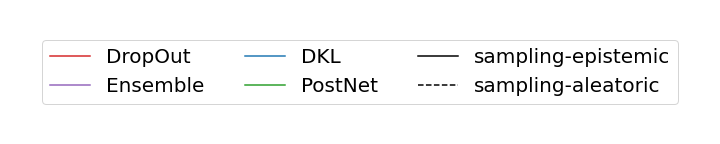
\includegraphics[width=\textwidth]{sections/011_icml2022/resources/sampling-legend.png}
    \end{subfigure}
    \vspace{-4mm}
    
    \begin{subfigure}{.23\textwidth}
        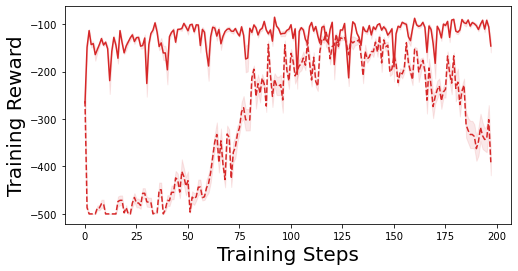
\includegraphics[width=\textwidth]{sections/011_icml2022/resources/acrobot-training_total_reward-dropout-training-strategy.png}
    \end{subfigure}
    \begin{subfigure}{.23\textwidth}
        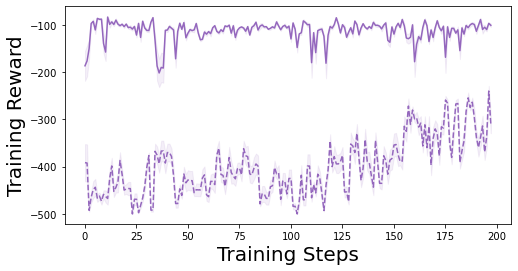
\includegraphics[width=\textwidth]{sections/011_icml2022/resources/acrobot-training_total_reward-ensemble-training-strategy.png}
    \end{subfigure}
    \begin{subfigure}{.23\textwidth}
        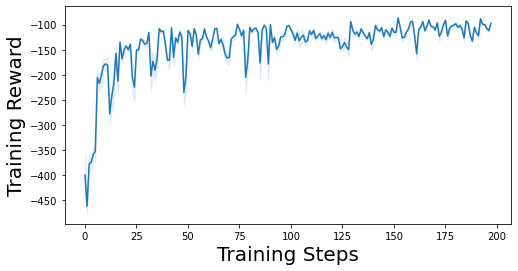
\includegraphics[width=\textwidth]{sections/011_icml2022/resources/acrobot-training_total_reward-dkl-training-strategy.png}
    \end{subfigure}
    \begin{subfigure}{.23\textwidth}
        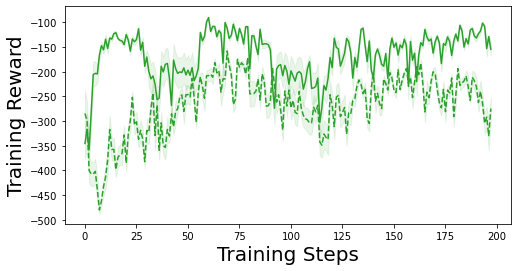
\includegraphics[width=\textwidth]{sections/011_icml2022/resources/acrobot-training_total_reward-postnet-training-strategy.png}
    \end{subfigure}
    
    % \begin{subfigure}{.245\textwidth}
    %     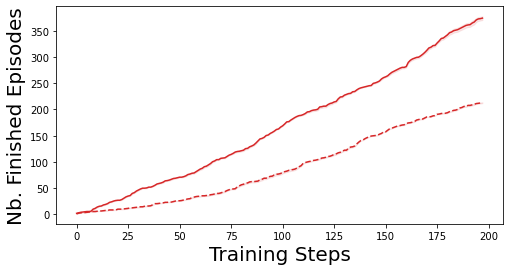
\includegraphics[width=\textwidth]{resources/acrobot-n_finished_training_episodes-dropout-training-strategy.png}
    % \end{subfigure}
    % \begin{subfigure}{.245\textwidth}
    %     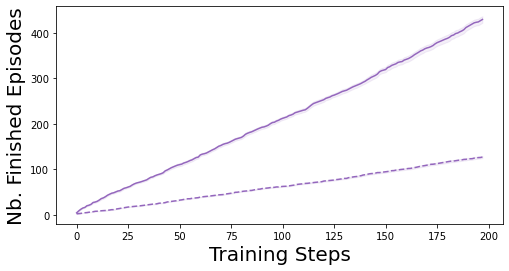
\includegraphics[width=\textwidth]{resources/acrobot-n_finished_training_episodes-ensemble-training-strategy.png}
    % \end{subfigure}
    % \begin{subfigure}{.245\textwidth}
    %     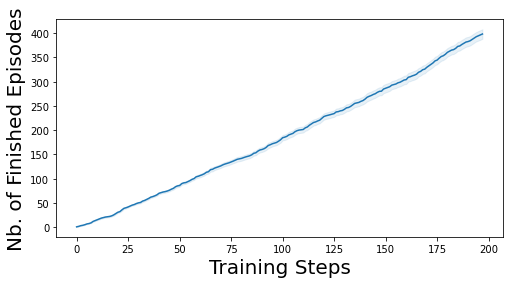
\includegraphics[width=\textwidth]{resources/acrobot-n_finished_training_episodes-dkl-training-strategy.png}
    % \end{subfigure}
    % \begin{subfigure}{.245\textwidth}
    %     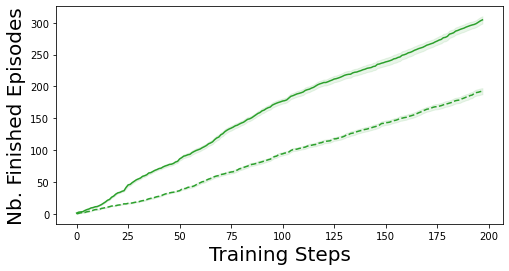
\includegraphics[width=\textwidth]{resources/acrobot-n_finished_training_episodes-postnet-training-strategy.png}
    % \end{subfigure}
    \vspace{-3mm}
    \caption{Comparison of the training performance on Acrobot. The four uncertainty methods use the sampling-aleatoric or the sampling-epistemic at training time. Ideally, an uncertainty aware-model should high reward with few samples.}
    \label{fig:strategy-training-performance-acrobot-main}
    \vspace{-5mm}
\end{figure*}